\documentclass[]{beamer}
\usetheme{Warsaw}
\usecolortheme{wolverine}
\usepackage[T1]{fontenc}
\usepackage[utf8]{inputenc}
\usepackage{lmodern}
\usepackage[ngerman]{babel}
\title{Krautspace -- Der Hackerspace in Jena}
\author{Frank Lanitz \\ \& \\Konrad Schöbel}
\date{\today}
\begin{document}
\frame{\titlepage}
\begin{frame}
	\begin{block}{zusammen gesetzt}
		\centering{}
		Hackerspace = Hacker + Space
	\end{block}
	\pause{}
	\begin{block}{Hacker}
		\begin{itemize}
			\item Jemand, der bekannte Sachen auseinandernimmt, versteht 
				und (krativ) neu zusammen setzt
			\item \dots{} der Spaß an kreativem Umgang mit Technik hat.
		\end{itemize}
	\end{block}
	\pause{}
	\begin{block}{Space}
		\begin{itemize}
			\item Ein physikalischer Raum für Hacker
		\end{itemize}
	\end{block}
\end{frame}
\begin{frame}
	\frametitle{Was ist ein Hackerspace}
	\begin{block}{}
		Ein Hackerspace ist \dots{} \\	
		\dots{} ein „Infrastrukturprovider“:
		\begin{itemize}
			\item Raum
			\item Strom
			\item Internet
			\item Kontakte
			\item Werkzeuge und Bauteile
			\item Essen \& Trinken	
		\end{itemize}
	\end{block}
\end{frame}
\begin{frame}
	\begin{block}{In einem Hackerspace gibt es \dots{}}
	\begin{itemize}
			\item Do-It-Yourself
			\item Vorträge
			\item Workshops
			\item Diskussionen
			\item Zocken
			\item Parties
		\end{itemize}
	\end{block}
	\begin{block}{Themen}
		\begin{itemize}
			\item Hardware
			\item Software
			\item Gesellschaft \& Technologie
			\item Kunst
		\end{itemize}
	\end{block}
\end{frame}
\begin{frame}
	\frametitle{Veranstaltungen}
	\begin{block}{Rückblick}
		\begin{itemize}
			\item Anfang Oktober: Hackerfahrschule 
				(Tor, Linux, \LaTeX{}, git, \texttt{/bin/sh}, vi vs emacs)
			\item DIY Kochrunden (Nudeln, Chili)
		\end{itemize}
	\end{block}
	\begin{block}{Voraussschau}
		\begin{itemize}
			\item Regelmäßig:
				\begin{itemize}
					\item Jeden Dienstag offene Runde mit 0xAFFE
					\item Jeden zweiten Donnerstag Stammtisch der \\
						\textbf{L}inux-\textbf{U}ser-\textbf{G}roup Jena
					\item Jeden zweiten Sonntag Chaoscafe
				\end{itemize}
			\item 24.10 20h: Einführung in Gentoo-Linux
			\item 15.11 18:30: Vortrag von Matthias Kirschner (FSFE):  \\
				\textit{Vom Aussterben bedroht: Die Universalmaschine Computer}
		\end{itemize}	
	\end{block}
\end{frame}
\begin{frame}
	\frametitle{Location}
	Hier können wir gefunden werden: 
	\begin{columns}[c]
		\column[c]{5cm}
			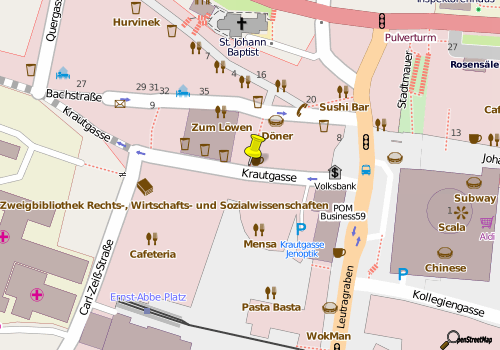
\includegraphics[width=5cm]{media/oss_location.png}
		\column[c]{5cm}
			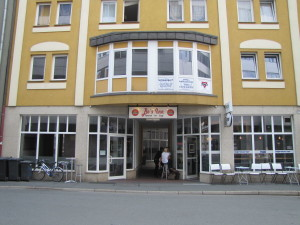
\includegraphics[width=5cm]{media/durchgang_zum_space.jpg}
	\end{columns}
\end{frame}
\begin{frame}
	\frametitle{Kontakt}
	\begin{block}{}
		\begin{description}
			\item[homepage] \url{https://www.hackspace-jena.de}
			\item[Mailingliste] \url{http://yaturl.net/0d3a}
			\item[Jabber] \url{xmapp://hackspace@chat.lug-jena.de}
			\item[Twitter] @HackspaceJena
			\item[identi.ca] @HackspaceJena
			% Wir machen keine Facebookwerbung im. Bitte sehr vorsichtig sein, 
			% beim einkommentieren
			% \item[facebook] \url{http://www.facebook.com/HackspaceJena}
		\end{description}
	\end{block}
\end{frame}
\end{document}
